\documentclass[11pt]{article}

\usepackage[margin=1in]{geometry}
\usepackage{amsmath}
\usepackage{amssymb}
\usepackage{booktabs}
\usepackage{caption}
\usepackage{enumitem}
\usepackage{hyperref}
\usepackage{microtype}
\usepackage{placeins}
\usepackage{pgfplots}
\usepackage{xcolor}

\pgfplotsset{
  compat=1.18,
  every axis/.append style={
    scaled ticks=false,
    tick label style={/pgf/number format/fixed,/pgf/number format/precision=2}
  },
  every node near coord/.append style={
    /pgf/number format/fixed,
    /pgf/number format/precision=2
  }
}
\hypersetup{
  colorlinks=true,
  linkcolor=blue!45!black,
  urlcolor=blue!45!black,
  citecolor=blue!45!black
}

\definecolor{PlotNavy}{HTML}{2F5D8C}
\definecolor{PlotTeal}{HTML}{2A9D8F}
\definecolor{PlotGold}{HTML}{E9A23B}
\definecolor{PlotRed}{HTML}{C94C4C}
\definecolor{PlotGray}{HTML}{747474}
\definecolor{PlotLightGray}{HTML}{D9D9D9}

\title{When Decodable Beliefs Do Not Drive Actions:\\
Evidence for a Belief--Action Gap in GPT-OSS-20B Gridworld Agents}
\author{Anonymous Authors}
\date{May 5, 2026}

\begin{document}
\maketitle

\begin{abstract}
We study a belief--action gap in a language-model gridworld agent: the model's hidden states can encode task-relevant beliefs or optimal actions, while the sampled action emitted by the model does not reliably follow that encoded information.
Across several related experiments, the evidence is consistent and more nuanced than a simple ``belief is causal'' or ``belief is epiphenomenal'' answer.
In fixed four-room and Seed12 trajectory datasets, hidden activations predict A* or BFS-optimal actions far better than they predict the model's observed actions, even though observed actions are often suboptimal.
However, clean full-vector activation swaps of a \texttt{carrying\_key} belief in a verbose door-key prompt do not flip action selection once prompt confounds are removed.
Additive steering along a learned \texttt{has\_key} direction does produce clean bidirectional action control in matched final-channel prompt families, but this effect is layer-specific: it appears at layer 23, not at layers 7 or 15 under the same sweep.
A stricter Seed12 desired-vs-wrong control shows a separate targeted causal effect at layer 15 when the steering direction is the raw probe-logit margin from the model's actual no-hook baseline action to the desired optimal action.
A matched layer-23 retry of the same Seed12 protocol fails at the layer-15 scale and across positive high-alpha screens, but an extreme opposite-sign layer-23 stress test produces a weaker replicated desired-vs-wrong effect.
The central conclusion is that decodability alone is not evidence that a belief is load-bearing for action.
Belief-to-action causality depends on the prompt family, layer, token positions, intervention type, and whether the intervention is aligned with the model's actual baseline action.
\end{abstract}

\section{Introduction}

This paper studies a failure mode in language-model agents: internal representations can encode task-relevant information even when the model's emitted action does not use that information reliably.
In a gridworld, for example, a model may internally represent that it has a key, or that a particular move is shortest-path optimal, while still sampling a nonoptimal action.
We call this mismatch the \emph{belief--action gap}.
The term is intended operationally rather than philosophically: it names a measurable separation between representation, intervention, and behavior.

The phrase has two meanings in this paper.
First, there is a \emph{behavioral gap}: the optimal action is linearly or nonlinearly decodable from internal activations, but the sampled action is often not optimal.
Second, there is a \emph{causal gap}: even when a belief or action variable is decodable, intervening on that representation at one layer and position does not necessarily move the emitted action in the corresponding direction.
This distinction matters because a probe can read a feature that is correlated with the decision process without that feature being read by the action pathway.

The central methodological lesson is that a changed final action is not sufficient evidence of causal desired steering.
A perturbation can change output by damaging the computation, by increasing randomness, or by moving probability mass toward an arbitrary alternative action.
The stronger causal claim must be directional: the intervention should move the action toward the intended target more than comparable wrong-target interventions do.
The later Seed12 steering experiment therefore uses a desired-vs-wrong control as its main criterion.

\paragraph{Contributions.}
This paper makes four contributions.
First, it synthesizes probing, activation-patching, additive-steering, and IRL-style behavioral analyses under one belief--action-gap framework.
Second, it shows that hidden states in fourroom and Seed12 gridworld agents encode optimal actions more strongly than observed behavior would suggest.
Third, it separates decodability from causal use: a corrected full-vector \texttt{carrying\_key} swap is null in a verbose prompt, while matched final-channel prompts are steerable.
Fourth, it introduces a stricter desired-vs-wrong criterion for action steering and applies it to Seed12, where source-aligned target-minus-baseline-action margins pass the test in a clean layer-15 regime and a weaker extreme layer-23 regime.

\section{Experimental Setting}

All experiments are gridworld decision tasks involving four actions: LEFT, RIGHT, UP, and DOWN.
The main model is GPT-OSS-20B, run either through the original trajectory-generation setup or through MLX for local activation intervention with \texttt{mlx-community/gpt-oss-20b-MXFP4-Q4}.
The environments include fixed four-room door-key layouts, synthetic final-channel prompt families, and real Seed12 trajectory-step prompts.

The shared task structure is simple but diagnostic.
The agent must navigate walls, collect a key when needed, open a locked door, and reach a goal.
This creates states where a latent task variable such as \texttt{has\_key} changes the optimal action even when the rendered grid location is otherwise similar.
It also creates many opportunities for a model to know the task structure but emit a nonoptimal sampled action.

\section{Related Work}

The paper builds on three methodological traditions.
First, linear probes and diagnostic classifiers are widely used to ask whether information is accessible in neural activations \cite{alain2016,belinkov2022,hewitt2019}.
The belief--action gap is precisely a case where accessibility is not the same as causal use: a probe may succeed even when the model's behavior does not follow the probed variable.

Second, causal intervention methods replace or edit internal activations to test whether a representation is load-bearing for downstream behavior \cite{meng2022,pearl2009}.
The flag-swap experiments use full-vector replacement, while the steering experiments use additive directions.
The desired-vs-wrong control follows the same causal logic: an intervention must change behavior in the direction predicted by the hypothesized variable, not merely change behavior.

Third, activation steering and activation addition show that learned or hand-selected directions can sometimes control model behavior without retraining \cite{turner2023}.
The final-channel and Seed12 experiments extend this idea to a gridworld action setting, where success can be judged against environment-defined optimal actions.
The fixed-grid MaxEnt IRL experiment connects the same agent behavior to a reward-modeling view of long-horizon key-door-goal structure \cite{ziebart2008}.

\begin{table}[t]
\centering
\caption{Experiments synthesized in this paper.}
\label{tab:experiments}
\begin{tabular}{p{0.24\linewidth} p{0.34\linewidth} p{0.30\linewidth}}
\toprule
Experiment & Primary question & Main result \\
\midrule
Fourroom action-vs-optimal probes & Do layer-15 prompt-suffix activations predict observed actions or BFS-optimal actions? & Optimal-action labels are predicted at 96.0\% accuracy; observed agent labels are predicted at 45.4\%, below the 54.8\% majority baseline. \\
Seed12 action probes & Does action information remain decodable under a larger real trajectory-step sweep and a state-held-out variant? & State-averaged optimal-action probe reaches 79.31\%; recorded actions are optimal only 12.72\% of the time. \\
Flag-swap activation patching & Is the layer-15 \texttt{carrying\_key} suffix residual causally load-bearing in a verbose door-key prompt? & Earlier positive-looking effects track prompt confounds; the corrected clean swap is null. \\
Final-channel \texttt{has\_key} steering & Can a learned belief direction causally steer immediate action tokens in matched prompt families? & Layer-23 additive steering flips actions bidirectionally in simple-corridor and 9x9 door-key final-channel prompts; the same criterion fails at layers 7 and 15. \\
Seed12 desired action steering & Does an optimal-action probe direction move real Seed12 outputs toward a desired action rather than merely changing actions? & A raw target-minus-baseline-action margin at layer 15 gives a +0.159 desired-vs-wrong conversion advantage; layer 23 is inert at matched/positive scales but gives a weaker +0.106 confirmation at $\alpha=-1024$. \\
\bottomrule
\end{tabular}
\end{table}

\section{Methodology}

\subsection{Notation}

Table~\ref{tab:notation} defines the symbols used in the pseudocode.
When a symbol has a different role in one experiment, the algorithm explicitly redefines it.
The model parameters are never updated in these experiments; only probes, reward weights, or intervention vectors are fit or applied.

\begin{table}[t]
\centering
\small
\caption{Common notation used by the experimental algorithms.}
\label{tab:notation}
\begin{tabular}{p{0.17\linewidth} p{0.73\linewidth}}
\toprule
Symbol & Meaning \\
\midrule
$\mathcal{A}$ & Discrete action set, $\{\mathrm{LEFT},\mathrm{RIGHT},\mathrm{UP},\mathrm{DOWN}\}$. \\
$M_\theta$ & Frozen GPT-OSS-20B model with parameters $\theta$. The experiments read or edit activations but do not train $\theta$. \\
$x_i$ & Prompt or trajectory-step input for sample $i$. It contains the rendered grid, task text, and suffix tokens used before generation. \\
$s_i$ & Environment state for sample $i$, such as agent position, key flag, and door flag. In the IRL algorithm, $s$ also ranges over all reachable states. \\
$a_i^{\mathrm{true}}$ & Recorded action emitted by the model in the original trajectory for sample $i$. This is behavior, not an optimality label. \\
$A_i^*$ & Set of optimal actions for state $s_i$, computed by BFS or A*. It may contain more than one action when actions tie. \\
$h_{\ell,p}(x_i)$ & Activation vector from model layer $\ell$ at token position or pooled position group $p$ for input $x_i$. \\
$P_{\mathrm{suf}}$ & The final three prompt-suffix token positions used by the suffix probes and steering hooks. \\
$\bar{h}_{\ell,P}(x_i)$ & Mean-pooled activation over position set $P$: $\bar{h}_{\ell,P}(x_i)=|P|^{-1}\sum_{p\in P}h_{\ell,p}(x_i)$. \\
$W,b$ & Linear probe weight matrix and bias. The probe logits are $z(h)=Wh+b$. \\
$w_a$ & Row of $W$ corresponding to action or class $a$. \\
$\sigma$ & Feature-wise standard deviation used by the probe's activation scaler. \\
$\tilde{w}_a$ & Activation-space probe weight for action $a$: $\tilde{w}_a=w_a/\sigma$. Division is elementwise. \\
$d$ & Unit-norm steering direction in activation space. Different algorithms define $d$ as a class direction or a target-minus-source margin. \\
$\alpha$ & User-chosen steering strength multiplier. \\
$g$ & Empirical class-gap scale, usually a mean projection difference along $d$. \\
$\Delta h$ & Additive activation update applied by a hook, usually $\Delta h=\alpha g d$. \\
$\mathrm{Parse}(\cdot)$ & Deterministic parser mapping generated text to an action in $\mathcal{A}$ or to PARSE\_FAIL. \\
$y$ & Parsed action emitted by the current generation. \\
$c$ & Candidate target action considered by a steering control. \\
$t$ & Desired target action, usually an action in $A_i^*$. \\
$a_{\mathrm{src}}$ & Source action produced by a paired no-hook baseline; steering tries to move away from this action. \\
\bottomrule
\end{tabular}
\end{table}
\FloatBarrier

\subsection{Pseudocode Algorithms}

\noindent\textbf{Algorithm 1: Fourroom action-vs-optimal probe experiment.}
\begin{enumerate}[leftmargin=*,itemsep=1pt,topsep=2pt]
  \item Build a dataset $\mathcal{D}=\{(x_i,s_i,a_i^{\mathrm{true}},A_i^*)\}_{i=1}^{N}$ from the fixed fourroom trajectories.
  \item For each sample $i$, extract $\bar{h}_{15,P_{\mathrm{suf}}}(x_i)$, the layer-15 prompt-suffix activation pooled over the final three suffix positions.
  \item Create two labelings of the same activation dataset: observed-action labels $a_i^{\mathrm{true}}$ and optimal-action labels $A_i^*$.
  \item Split records into train and test sets.
  \item Train probe $f_{\mathrm{true}}(h)=\arg\max_a (W_{\mathrm{true}}h+b_{\mathrm{true}})_a$ on observed-action labels.
  \item Train probe $f_{\mathrm{opt}}(h)=\arg\max_a (W_{\mathrm{opt}}h+b_{\mathrm{opt}})_a$ on optimal-action labels.
  \item Evaluate $f_{\mathrm{true}}$ by exact match against $a_i^{\mathrm{true}}$.
  \item Evaluate $f_{\mathrm{opt}}$ by membership: success if $f_{\mathrm{opt}}(h_i)\in A_i^*$.
  \item Compare probe accuracy to the behavioral optimality rate $\frac{1}{N}\sum_i \mathbf{1}[a_i^{\mathrm{true}}\in A_i^*]$.
\end{enumerate}
\noindent\emph{Algorithm-specific symbols.}
$N$ is the number of usable trajectory steps.
$f_{\mathrm{true}}$ is the probe trained to predict what the model actually did.
$f_{\mathrm{opt}}$ is the probe trained to predict what the environment planner says is optimal.
$\mathbf{1}[\cdot]$ is an indicator that equals 1 when its condition is true and 0 otherwise.

\medskip
\noindent\textbf{Algorithm 2: Seed12 step-level and state-averaged action probe sweep.}
\begin{enumerate}[leftmargin=*,itemsep=1pt,topsep=2pt]
  \item Build trajectory-step dataset $\mathcal{D}_{\mathrm{step}}=\{(x_i,s_i,a_i^{\mathrm{true}},A_i^*)\}_{i=1}^{N}$ from Seed12.
  \item For each layer $\ell\in\{7,15,23\}$ and position family $p$:
    \begin{enumerate}[leftmargin=1.5em,itemsep=1pt,topsep=1pt]
      \item Extract activation feature $h_{\ell,p}(x_i)$ or a mean-pooled feature $\bar{h}_{\ell,P}(x_i)$.
      \item Train linear and MLP probes for true-action labels $a_i^{\mathrm{true}}$.
      \item Train linear and MLP probes for optimal-action labels $A_i^*$.
      \item Evaluate true-action probes by balanced accuracy against $a_i^{\mathrm{true}}$.
      \item Evaluate optimal-action probes by top-1 membership in $A_i^*$.
    \end{enumerate}
  \item For the state-averaged variant, group samples by state key $k(s_i)$.
  \item Replace all activations in a group with $\bar{h}_{k}=\frac{1}{|\mathcal{I}_k|}\sum_{i\in\mathcal{I}_k}h_i$, where $\mathcal{I}_k=\{i:k(s_i)=k\}$.
  \item Require labels to agree within each group; otherwise reject the group as ambiguous.
  \item Split by held-out state keys and repeat the probe training/evaluation sweep.
\end{enumerate}
\noindent\emph{Algorithm-specific symbols.}
$p$ denotes one saved position family, such as pre-reasoning suffix, CoT rank, or post-reasoning tail.
$k(s_i)$ is the discrete state key, including position and inventory/door flags.
$\mathcal{I}_k$ is the set of indices sharing the same state key.
$\bar{h}_{k}$ is the state-averaged activation used to reduce repeated-state leakage.

\medskip
\noindent\textbf{Algorithm 3: Corrected flag-swap full-vector activation patch.}
\begin{enumerate}[leftmargin=*,itemsep=1pt,topsep=2pt]
  \item Construct two prompts with identical grid and prefix semantics:
    $x^0$ for no-key and $x^1$ for has-key.
    The only semantic suffix difference is \texttt{Carrying key: False} versus \texttt{Carrying key: True}.
  \item Capture donor tensors $H^0=\{h_{15,p}(x^0):p\in P_{\mathrm{suf}}\}$ and $H^1=\{h_{15,p}(x^1):p\in P_{\mathrm{suf}}\}$.
  \item For each condition in $\{\mathrm{baseline}\text{-}0,\mathrm{self}\text{-}0,\mathrm{swap}\text{-}0{\leftarrow}1,\mathrm{baseline}\text{-}1,\mathrm{self}\text{-}1,\mathrm{swap}\text{-}1{\leftarrow}0\}$:
    \begin{enumerate}[leftmargin=1.5em,itemsep=1pt,topsep=1pt]
      \item Select prompt $x^0$ or $x^1$.
      \item Select hook mode: no replacement, replace with its own tensor, or replace with the opposite tensor.
      \item Generate $R$ sampled completions at temperature 0.7.
      \item Parse each completion with $\mathrm{Parse}$ and count action frequencies.
    \end{enumerate}
  \item Test the directional prediction: $\mathrm{swap}\text{-}0{\leftarrow}1$ should increase UP frequency, and $\mathrm{swap}\text{-}1{\leftarrow}0$ should decrease UP frequency.
  \item Compare each swap against its self-control using action distributions and $\chi^2$ tests.
\end{enumerate}
\noindent\emph{Algorithm-specific symbols.}
$x^0$ and $x^1$ are the two corrected prompts.
$H^0$ and $H^1$ are full residual-stream donor tensors, not probe directions.
$R$ is the number of sampled completions per condition.
The self-control checks whether hook plumbing alone changes behavior.

\medskip
\noindent\textbf{Algorithm 4: Final-channel \texttt{has\_key} additive steering.}
\begin{enumerate}[leftmargin=*,itemsep=1pt,topsep=2pt]
  \item Build paired final-channel prompts $\{(x_j^0,x_j^1)\}_{j=1}^{m}$, where $x_j^0$ is no-key and $x_j^1$ is has-key.
  \item For each layer $\ell\in\{7,15,23\}$, extract suffix features over $P_{\mathrm{suf}}$ and train a linear \texttt{has\_key} probe.
  \item Convert normalized probe weights to activation-space weights: $\tilde{w}_{\mathrm{key}}=w_{\mathrm{key}}/\sigma$.
  \item Define unit direction $d_{\mathrm{key}}=\tilde{w}_{\mathrm{key}}/\|\tilde{w}_{\mathrm{key}}\|_2$.
  \item Estimate class gap $g=\mathbb{E}[h\cdot d_{\mathrm{key}}\mid \mathrm{has\_key}=1]-\mathbb{E}[h\cdot d_{\mathrm{key}}\mid \mathrm{has\_key}=0]$.
  \item For each target prompt, layer $\ell$, and steering strength $\alpha$:
    \begin{enumerate}[leftmargin=1.5em,itemsep=1pt,topsep=1pt]
      \item Add $\Delta h=\alpha g d_{\mathrm{key}}$ to each suffix position in $P_{\mathrm{suf}}$ during prompt processing.
      \item Generate $R$ final-channel action completions.
      \item Parse actions and measure whether the action moves in the predicted key-state direction.
    \end{enumerate}
  \item Declare a clean steering result only if positive and negative $\alpha$ produce the expected bidirectional action flips and hook logs show exactly $P_{\mathrm{suf}}$ was patched.
\end{enumerate}
\noindent\emph{Algorithm-specific symbols.}
$m$ is the number of paired synthetic prompt templates.
$d_{\mathrm{key}}$ is the learned direction for increasing the \texttt{has\_key} belief.
$g$ scales a unit direction by the empirical separation between no-key and has-key activations.

\medskip
\noindent\textbf{Algorithm 5: Seed12 desired-vs-wrong optimal-action steering.}
\begin{enumerate}[leftmargin=*,itemsep=1pt,topsep=2pt]
  \item Prepare activation-space action weights $\tilde{w}_a=w_a/\sigma$ for every action $a\in\mathcal{A}$ from the Seed12 optimal-action linear probe.
  \item For each eligible Seed12 step $i$, reconstruct prompt $x_i$ from prefix, rendered grid, and step-specific suffix.
  \item Generate a no-hook baseline using sample seed $r$ and parse it: $a_{\mathrm{src}}=\mathrm{Parse}(M_\theta(x_i;r))$.
  \item Skip the pair if $a_{\mathrm{src}}=\mathrm{PARSE\_FAIL}$ or $a_{\mathrm{src}}\in A_i^*$.
  \item For each candidate action $c\in\mathcal{A}\setminus\{a_{\mathrm{src}}\}$:
    \begin{enumerate}[leftmargin=1.5em,itemsep=1pt,topsep=1pt]
      \item Define margin direction
      \[
        d_{c,a_{\mathrm{src}}}
        =
        \frac{\tilde{w}_c-\tilde{w}_{a_{\mathrm{src}}}}
        {\|\tilde{w}_c-\tilde{w}_{a_{\mathrm{src}}}\|_2}.
      \]
      \item Compute candidate gap $g_c$ from the target class's mean activation separation projected onto $d_{c,a_{\mathrm{src}}}$.
      \item Add $\Delta h=\alpha g_c d_{c,a_{\mathrm{src}}}$ at the selected test layer $\ell_{\mathrm{test}}$ and positions $P_{\mathrm{suf}}$.
      \item Regenerate with the same prompt $x_i$ and seed $r$; parse the hooked action $y_{i,c}$.
      \item Mark $c$ as desired if $c\in A_i^*$; otherwise mark it as a wrong-target control.
    \end{enumerate}
  \item Estimate desired conversion rate $\Pr[y_{i,c}=c\mid c\in A_i^*]$ and wrong-control conversion rate $\Pr[y_{i,c}=c\mid c\notin A_i^*]$.
  \item Claim desired steering only if desired conversion is positive and exceeds wrong-control conversion under paired prompt/seed/source comparisons.
\end{enumerate}
\noindent\emph{Algorithm-specific symbols.}
$r$ is the random generation seed.
$\ell_{\mathrm{test}}$ is the layer being intervened on; the successful confirmation uses $\ell_{\mathrm{test}}=15$, while the later layer-23 retry uses the same algorithm with $\ell_{\mathrm{test}}=23$.
$a_{\mathrm{src}}$ is the actual no-hook action that the intervention tries to move away from.
$c$ is any candidate target action.
$y_{i,c}$ is the parsed action after steering toward candidate $c$.
The comparison is paired because $x_i$, $r$, and $a_{\mathrm{src}}$ are shared across desired and wrong candidates.

\medskip
\noindent\textbf{Algorithm 6: Fixed-grid n-step MaxEnt IRL side experiment.}
\begin{enumerate}[leftmargin=*,itemsep=1pt,topsep=2pt]
  \item Define reachable state space $\mathcal{S}$ for the fixed 13x13 grid, where each state $s\in\mathcal{S}$ includes agent position, key flag, and door flag.
  \item Define deterministic transition function $T(s,a)$ for every state-action pair $(s,a)$.
  \item Build feature vector $\phi(s)$ containing distances to goal/key/door and binary key/door indicators.
  \item Initialize reward weights $\Theta$ and reward $R_\Theta(s)=\Theta^\top\phi(s)$.
  \item Compute empirical feature mean $\hat{\phi}_{\mathrm{demo}}$ from demonstration states.
  \item Repeat for each training epoch:
    \begin{enumerate}[leftmargin=1.5em,itemsep=1pt,topsep=1pt]
      \item Run $H$ soft Bellman backups:
      \[
        Q(s,a)=R_\Theta(s)+V(T(s,a)),\qquad
        V(s)=\log\sum_{a\in\mathcal{A}}\exp Q(s,a).
      \]
      \item Extract policy
      \[
        \pi_\Theta(a\mid s)=
        \frac{\exp Q(s,a)}
        {\sum_{a'\in\mathcal{A}}\exp Q(s,a')}.
      \]
      \item Propagate state visitation $\mu_\Theta(s)$ forward for $H$ steps from empirical initial states.
      \item Compute policy feature mean $\hat{\phi}_{\mathrm{policy}}=\sum_{s\in\mathcal{S}}\mu_\Theta(s)\phi(s)$.
      \item Update reward weights $\Theta\leftarrow\Theta+\eta(\hat{\phi}_{\mathrm{demo}}-\hat{\phi}_{\mathrm{policy}})$.
    \end{enumerate}
  \item Interpret $\Theta$ as the reward weights that make the MaxEnt policy match demonstration feature expectations.
\end{enumerate}
\noindent\emph{Algorithm-specific symbols.}
$\mathcal{S}$ is the reachable state set.
$T$ is the deterministic environment transition.
$\phi(s)$ is the hand-crafted feature vector.
$\Theta$ is the learned reward-weight vector, distinct from the frozen model parameters $\theta$.
$R_\Theta$ is the scalar reward, $Q$ is the soft action value, $V$ is the soft state value, $\pi_\Theta$ is the induced policy, $\mu_\Theta$ is expected state visitation, $H$ is the planning horizon, and $\eta$ is the learning rate.

\subsection{Probing}

The probing experiments train lightweight supervised models on frozen activations.
For each sample, a feature vector $h_{\ell,p}$ is extracted from layer $\ell$ and position or pooled position group $p$.
The labels are either the model's recorded action, denoted $a_{\mathrm{true}}$, or an optimal-action set $A^*(s)$ computed by BFS or A* in the environment state space.
The probe is deliberately simple: it asks whether the information is available to a classifier, not whether the model itself uses that information.

For four-way single-label probes, a linear probe has logits
\[
  z(h) = W h + b,\quad W \in \mathbb{R}^{4 \times d}.
\]
For optimal-action probes with ties, success is measured by top-1 set membership: the predicted action is counted correct if it lies in $A^*(s)$.
For Seed12, the stricter state-averaged variant first groups trajectory steps by state key and averages activations within each state, then splits by held-out state keys.
This removes repeated-state leakage that can inflate step-level results.

\subsection{Full-Vector Activation Swap}

The flag-swap experiment captures the layer-15 residual stream at the final three prompt-suffix positions for two matched prompts:
a no-key prompt $a$ and a has-key prompt $b$.
The hook can pass through, replace a prompt with its own captured activations as a no-op control, or replace a prompt's captured positions with the other prompt's activations.
The causal prediction is directional:
\[
  \mathrm{swap}(a \leftarrow b) \text{ should increase UP frequency,}
\]
because the has-key state is optimal for going through the door, while
\[
  \mathrm{swap}(b \leftarrow a) \text{ should decrease UP frequency.}
\]
The final corrected run uses prompts that differ only in the rendered \texttt{True}/\texttt{False} key-state suffix token and removes a prompt contradiction that made earlier runs out of distribution.
This design is intentionally conservative: if an entire donor residual stream at the selected positions cannot move the action in the predicted direction, then a narrower subdirection at the same layer and positions has little support as a causal explanation in that prompt family.

\subsection{Additive Probe-Direction Steering}

For a linear probe trained with standardized features, the checkpoint weight is in normalized coordinates.
If the feature scaler has standard deviation vector $\sigma$, the activation-space action vector is
\[
  \tilde{w}_a = \frac{w_a}{\sigma}.
\]
The single-action direction is $d_a = \tilde{w}_a / \|\tilde{w}_a\|_2$.
For final-channel \texttt{has\_key} steering, the hook adds
\[
  \Delta h = \alpha \, g \, d
\]
to each of the final three suffix positions, where $g$ is the empirical class gap along the probe direction.
Adding the same vector to all three suffix positions matches the mean-pooled probe input: the mean activation shifts by exactly that vector.

\subsection{Desired-vs-Wrong Steering Criterion}

The Seed12 steering experiments use real trajectory-step prompts and sampled decoding at temperature 0.7.
The early steering metric, ``did the action change?'', is too weak.
The later criterion asks whether the intervention converts a baseline nonoptimal action into the desired optimal action more often than wrong candidate directions do.

The successful Seed12 variant uses the model's actual paired no-hook output as the source action.
If the baseline emits source action $s$ and the desired target is $t \in A^*(x)$, the direction is the raw probe-logit margin
\[
  d_{t,s} = \frac{\tilde{w}_t - \tilde{w}_s}{\|\tilde{w}_t - \tilde{w}_s\|_2}.
\]
Wrong controls use the same source $s$ but substitute non-desired candidate targets.
The support criterion is:
\[
  \mathrm{conversion}_{\mathrm{desired}} > 0
  \quad\text{and}\quad
  \mathrm{conversion}_{\mathrm{desired}} >
  \mathrm{conversion}_{\mathrm{wrong}}.
\]
This rejects interventions that merely perturb the model or make wrong directions fail even worse.
It also separates two distinct claims: \emph{optimality improvement}, where the output lands in $A^*(s)$, and \emph{true-action retention}, where the output matches the recorded trajectory action.
Those metrics can move in opposite directions because the recorded trajectory action is often not optimal.

\subsection{Seed12 Steering Algorithm}

For each eligible Seed12 step, the implementation reconstructs the exact prompt from the trajectory prefix, current grid, and step-specific suffix.
It resolves the final three suffix-token positions as absolute prompt positions, generates a no-hook baseline under a fixed sample seed, parses the emitted action, and only keeps samples whose baseline action is parseable and nonoptimal.
For each candidate target action other than the source, it adds the target-minus-source margin at a selected layer and regenerates with the same prompt and seed.
Rows record the true action, optimal set, baseline source, candidate target, whether the target is desired, emitted action, parse status, selected positions, and hook log.

The hook audit for the largest confirmation checked 207 hooked rows.
Every row selected exactly three positions, all relative to the suffix positions intended by the probe input, and no bad hook logs were found.
This matters because a positive effect would be much less interpretable if the hook were patching generated tokens or unrelated prompt positions.
The same hook-log audit passed for the layer-23 retry rows that record hook metadata.

\section{Results}

\subsection{Decodable Optimal Actions Outpace Observed Actions}

The first major result is representational.
In the fixed fourroom action-vs-optimal experiment, a linear layer-15 prompt-suffix probe trained on observed agent actions reaches only 45.4\% test accuracy, below the 54.8\% UP majority baseline.
The same architecture trained on BFS-optimal labels reaches 96.0\% test accuracy and 99.2\% optimal-set membership accuracy.
The dataset's observed agent action is optimal in only 32.5\% of kept transitions.

Seed12 reproduces the broader pattern in a larger and more varied real trajectory-step sweep.
Recorded parseable actions are optimal in only 406 of 3192 cases, or 12.72\%.
Step-level probes can reach near-ceiling accuracy, but those splits have repeated-state caveats.
The stricter state-averaged Seed12 variant is more informative: the best held-out-state optimal-action probe reaches 79.31\%, while the best true-action probe reaches 66.28\%.
The hidden state therefore contains more reliable information about what should be done than the model's observed behavior suggests.

\begin{figure}[t]
\centering
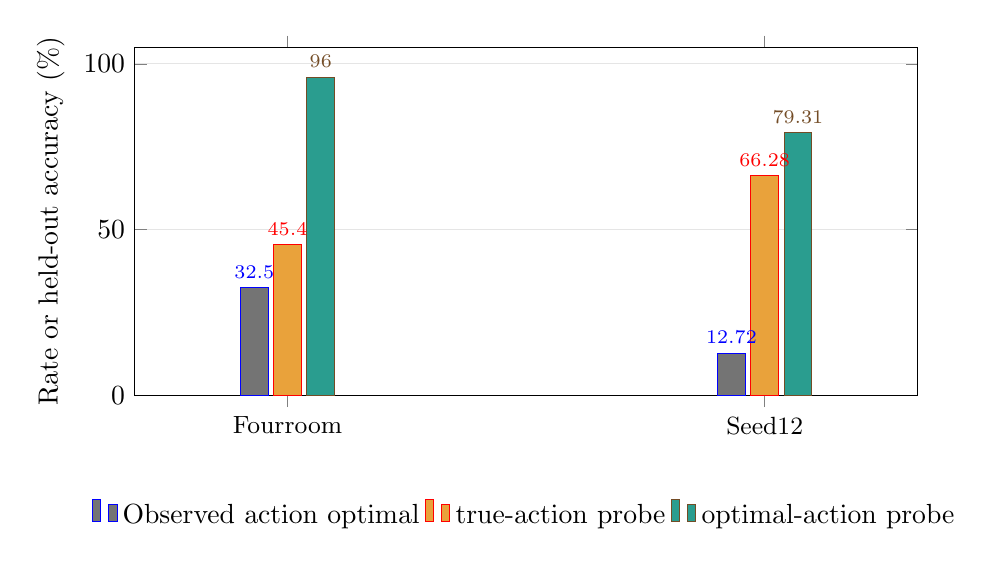
\begin{tikzpicture}
\begin{axis}[
  ybar,
  width=0.95\linewidth,
  height=6.0cm,
  ymin=0,
  ymax=105,
  ylabel={Rate or held-out accuracy (\%)},
  symbolic x coords={Fourroom,Seed12},
  xtick=data,
  xticklabels={Fourroom,Seed12},
  x tick label style={align=center,font=\small},
  bar width=10pt,
  enlarge x limits=0.32,
  legend style={draw=none,at={(0.5,-0.28)},anchor=north,legend columns=3},
  nodes near coords,
  nodes near coords style={font=\scriptsize},
  every axis plot/.append style={line width=0pt},
  ymajorgrids=true,
  grid style={draw=gray!20}
]
\addplot+[fill=PlotGray] coordinates {(Fourroom,32.5) (Seed12,12.72)};
\addplot+[fill=PlotGold] coordinates {(Fourroom,45.4) (Seed12,66.28)};
\addplot+[fill=PlotTeal] coordinates {(Fourroom,96.0) (Seed12,79.31)};
\legend{Observed action optimal, true-action probe, optimal-action probe}
\end{axis}
\end{tikzpicture}
\caption{Behavioral optimality is low, but optimal-action information is strongly decodable. Fourroom uses a fixed 9x9 layout and layer-15 prompt-suffix activations. Seed12 uses the stricter state-averaged held-out-state probe results for the probe bars.}
\label{fig:decodability}
\end{figure}
\FloatBarrier

\subsection{The Clean Flag-Swap Test Is Null}

The flag-swap experiment was designed as a causal test of whether the layer-15 prompt-suffix residual carrying the \texttt{carrying\_key} belief is read out by the action selection pathway.
The first two iterations looked partially positive, especially on the no-key prompt patched with has-key activations.
However, the early iterations had important prompt confounds.
The asymmetric run used an unrendered suffix placeholder, so the key-state text was not actually the intended \texttt{True}/\texttt{False} difference.
The symmetric run fixed the suffix but made prompt $b$ internally contradictory: the grid showed the key while the suffix said the key was already carried, contradicting the original prompt rules.

The corrected run rewrote the prefix so the key symbol stays visible regardless of inventory state.
Now the prompts are internally consistent and differ only at the suffix key-state token.
Under this cleanest setup, the full-vector swap no longer produces a directed action flip.
The a-side UP frequency changes from 0.200 in the self-control to 0.133 under swap, a difference of -0.067 rather than the predicted increase.
The b-side UP frequency changes from 0.400 to 0.333, also -0.067.
Pairwise $\chi^2$ tests against self-controls are null: $p=0.27$ for a-side and $p=0.45$ for b-side.

\begin{figure}[t]
\centering
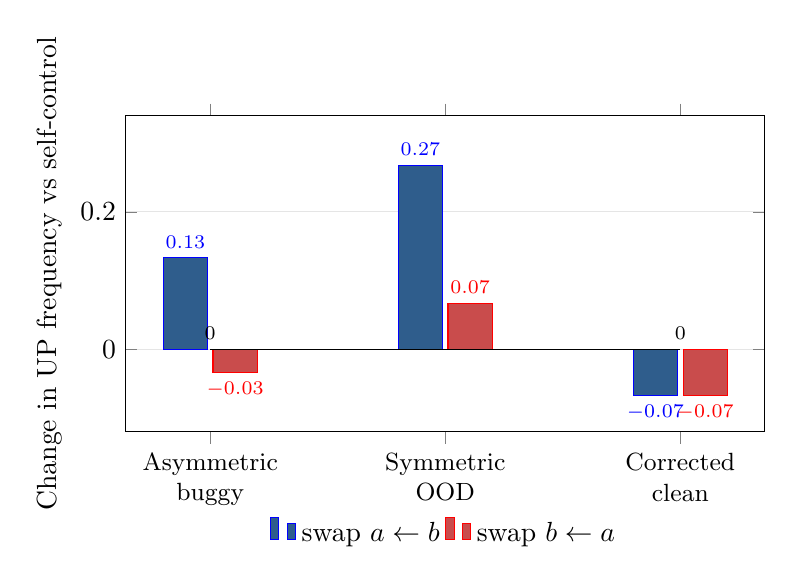
\begin{tikzpicture}
\begin{axis}[
  ybar,
  width=0.80\linewidth,
  height=5.6cm,
  ymin=-0.12,
  ymax=0.34,
  ylabel={Change in UP frequency vs self-control},
  symbolic x coords={Asym,Sym,Corr},
  xtick=data,
  xticklabels={Asymmetric\\buggy,Symmetric\\OOD,Corrected\\clean},
  x tick label style={align=center,font=\small},
  bar width=16pt,
  enlarge x limits=0.18,
  legend style={draw=none,at={(0.5,-0.25)},anchor=north,legend columns=2},
  nodes near coords,
  nodes near coords style={font=\scriptsize},
  ymajorgrids=true,
  grid style={draw=gray!20}
]
\addplot+[fill=PlotNavy] coordinates {(Asym,0.133) (Sym,0.267) (Corr,-0.067)};
\addplot+[fill=PlotRed] coordinates {(Asym,-0.033) (Sym,0.067) (Corr,-0.067)};
\addplot[black,sharp plot,update limits=false] coordinates {(Asym,0) (Corr,0)};
\legend{swap $a \leftarrow b$, swap $b \leftarrow a$}
\end{axis}
\end{tikzpicture}
\caption{The apparent flag-swap effect tracks prompt confounding. Once the prompt is corrected so the only remaining semantic difference is the key-state suffix token, full-vector layer-15 suffix swapping does not move actions in the predicted direction.}
\label{fig:flag_swap}
\end{figure}

This result is strong evidence against the simplest causal story at that layer and position.
It does not prove the key belief is never causal.
The causal pathway might use a different layer, the explicit \texttt{True}/\texttt{False} token itself, or later generated-token positions.
But it does show that a highly decodable suffix belief is not automatically load-bearing under a clean intervention.
\FloatBarrier

\subsection{Matched Final-Channel Prompts Are Steerable}

The final-channel steering experiments deliberately simplify the action interface.
Instead of a long verbose reasoning prompt where the model may generate substantial text before committing to an action, the prompt asks for the final action immediately.
In these prompt families, adding a learned \texttt{has\_key} direction to the last three suffix activations produces clean bidirectional control only at layer 23 among the tested layers.
The same intervention at layers 7 and 15 does not pass the clean steering criterion: it either leaves the baseline action largely unchanged, introduces noise or parse failures, or fails to produce the expected monotonic bidirectional pattern.

In the simple-corridor family, prompt A is no-key and emits DOWN at baseline; adding the positive \texttt{has\_key} direction at $\alpha=8$ changes it to UP in 30 of 30 samples.
Prompt B is has-key and emits UP at baseline; subtracting the direction at $\alpha=-8$ changes it to DOWN in 29 of 30 samples.
In the fixed 9x9 door-key final-channel family, prompt A changes from RIGHT=30/30 at baseline to UP=30/30 at $\alpha=4$ or $\alpha=8$, and prompt B changes from UP=30/30 to RIGHT=30/30 at $\alpha=-8$, $\alpha=-4$, and $\alpha=-2$.
Layer 23 is therefore not just the strongest tested layer; it is the only tested layer that gives the clean monotonic bidirectional pattern in both final-channel families.
The result should not be read as ``the \texttt{has\_key} direction works everywhere.''
It should be read as a localized causal result: final three suffix positions, final-channel prompts, additive \texttt{has\_key} direction, and layer 23.

\begin{figure}[t]
\centering
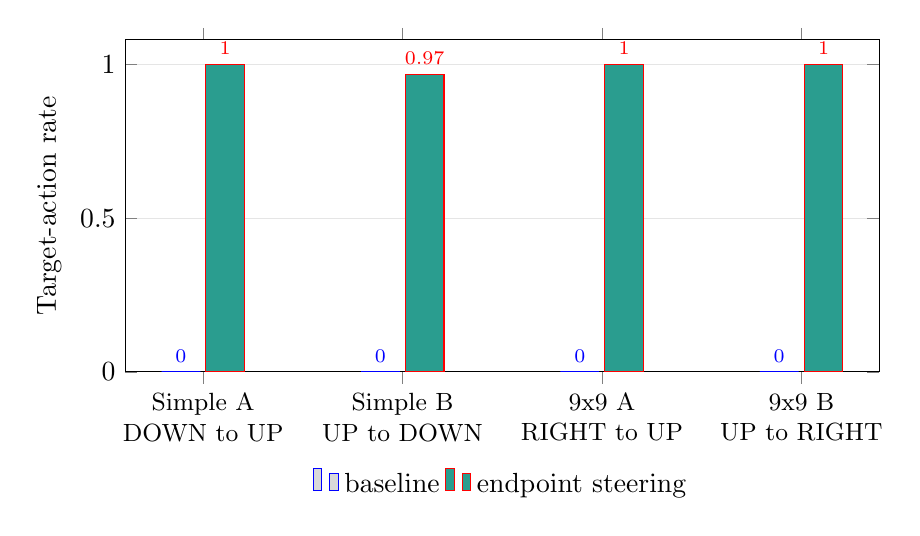
\begin{tikzpicture}
\begin{axis}[
  ybar,
  width=0.92\linewidth,
  height=5.8cm,
  ymin=0,
  ymax=1.08,
  ylabel={Target-action rate},
  symbolic x coords={SimpleA,SimpleB,GridA,GridB},
  xtick=data,
  xticklabels={Simple A\\DOWN to UP,Simple B\\UP to DOWN,9x9 A\\RIGHT to UP,9x9 B\\UP to RIGHT},
  x tick label style={align=center,font=\small},
  bar width=14pt,
  enlarge x limits=0.13,
  legend style={draw=none,at={(0.5,-0.27)},anchor=north,legend columns=2},
  nodes near coords,
  nodes near coords style={font=\scriptsize},
  ymajorgrids=true,
  grid style={draw=gray!20}
]
\addplot+[fill=PlotLightGray] coordinates {(SimpleA,0.0) (SimpleB,0.0) (GridA,0.0) (GridB,0.0)};
\addplot+[fill=PlotTeal] coordinates {(SimpleA,1.0) (SimpleB,0.967) (GridA,1.0) (GridB,1.0)};
\legend{baseline, endpoint steering}
\end{axis}
\end{tikzpicture}
\caption{Final-channel prompt families show clean bidirectional action control from a learned \texttt{has\_key} direction. The plotted target-action rate is the rate of the intended counterfactual action at the steering endpoint.}
\label{fig:final_channel}
\end{figure}

This positive result is not a contradiction of the flag-swap null.
It shows that a causal belief-to-action bridge exists when the prompt family, action channel, direction, layer, and positions are matched.
The verbose prompt may route action selection through later reasoning and explicit text tokens; the final-channel prompt makes the suffix representation immediately adjacent to the emitted action.
\FloatBarrier

\subsection{Seed12 Desired Steering Requires Source Alignment}

The Seed12 optimal-action steering experiment was the strictest causal test.
The first version added a target optimal-action probe direction to final three suffix positions.
That could change actions, but action change alone does not establish desired causal steering.
Several variants failed under the stricter desired-vs-wrong criterion:
target-only raw directions, action-vs-recorded-true directions, raw action-vs-recorded-true margins, and centroid action-vs-recorded-true margins were negative or did not pass strict support.

The successful variant uses the model's actual no-hook baseline action as the source.
For a baseline nonoptimal source action $s$ and desired optimal target $t$, the hook adds the raw margin direction $W_t - W_s$ at layer 15 with $\alpha=0.5$.
Wrong controls use the same source $s$ and the same prompt and seed, but target a non-desired candidate action.
In the largest confirmation, desired target directions convert 27 of 69 pairs to the desired action, or 39.1\%.
Wrong target controls convert 32 of 138 pairs, or 23.2\%.
The desired-vs-wrong advantage is therefore +0.159.

The same source-aligned protocol was then retried at layer 23, because the final-channel \texttt{has\_key} experiment had succeeded at layer 23.
At the matched layer-15 scale, this Seed12 layer-23 retry failed.
On the same balanced 12-step subset with $\alpha=0.5$, desired directions converted 0 of 58 pairs and wrong controls converted 0 of 116 pairs, giving a desired-vs-wrong advantage of 0.000.
A smaller stronger-alpha screen over $\alpha\in\{1,2,4,8\}$ also gave 0.000 desired conversion and 0.000 wrong-control conversion at every tested alpha.
A larger positive-alpha screen over $\alpha\in\{32,64,128,256,512\}$ also gave 0.000 desired conversion.
Across those positive layer-23 runs, all hooked outputs stayed equal to the paired no-hook source action.

A final sign stress test changed this picture.
At layer 23 with $\alpha=-1024$, the first screen converted 20.0\% of desired-direction pairs to an A*-optimal desired action, compared with 3.3\% for wrong-direction controls, for an advantage of +0.167.
An independent-seed confirmation replicated the effect: desired directions converted 24.2\% of pairs and wrong controls converted 13.6\%, for an advantage of +0.106.
The hook logs in this confirmation showed that the hook fired on exactly the final three suffix positions.
Thus the Seed12 action-margin result has two regimes: a cleaner moderate-scale layer-15 effect, and a weaker extreme opposite-sign layer-23 effect.
The latter is evidence that layer 23 can be causally effective, but not evidence that the matched positive layer-15 protocol transfers unchanged to layer 23.

\begin{figure}[t]
\centering
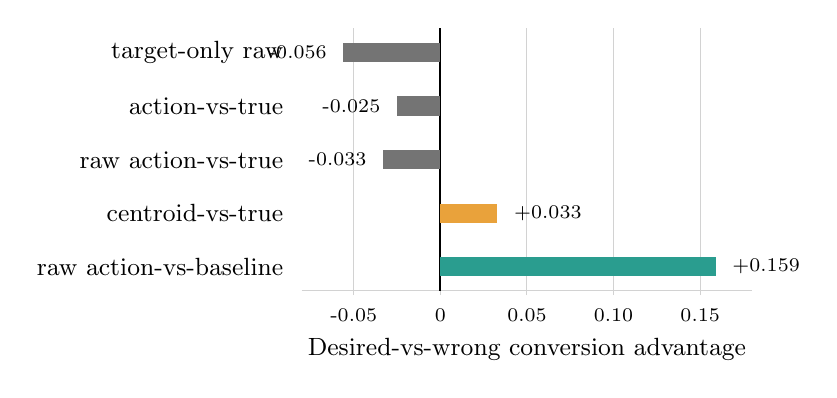
\begin{tikzpicture}[x=22cm,y=0.68cm]
  \draw[gray!35] (-0.08,-0.45) -- (0.18,-0.45);
  \foreach \x/\label in {-0.05/-0.05,0/0,0.05/0.05,0.10/0.10,0.15/0.15} {
    \draw[gray!35] (\x,-0.53) -- (\x,4.45);
    \node[font=\scriptsize,anchor=north] at (\x,-0.60) {\label};
  }
  \draw[black,line width=0.6pt] (0,-0.45) -- (0,4.45);
  \node[font=\small,anchor=north] at (0.05,-1.15) {Desired-vs-wrong conversion advantage};

  \node[font=\small,anchor=east] at (-0.085,4) {target-only raw};
  \draw[fill=PlotGray,draw=none] (0,3.82) rectangle (-0.056,4.18);
  \node[font=\scriptsize,anchor=east] at (-0.060,4) {-0.056};

  \node[font=\small,anchor=east] at (-0.085,3) {action-vs-true};
  \draw[fill=PlotGray,draw=none] (0,2.82) rectangle (-0.025,3.18);
  \node[font=\scriptsize,anchor=east] at (-0.029,3) {-0.025};

  \node[font=\small,anchor=east] at (-0.085,2) {raw action-vs-true};
  \draw[fill=PlotGray,draw=none] (0,1.82) rectangle (-0.033,2.18);
  \node[font=\scriptsize,anchor=east] at (-0.037,2) {-0.033};

  \node[font=\small,anchor=east] at (-0.085,1) {centroid-vs-true};
  \draw[fill=PlotGold,draw=none] (0,0.82) rectangle (0.033,1.18);
  \node[font=\scriptsize,anchor=west] at (0.037,1) {+0.033};

  \node[font=\small,anchor=east] at (-0.085,0) {raw action-vs-baseline};
  \draw[fill=PlotTeal,draw=none] (0,-0.18) rectangle (0.159,0.18);
  \node[font=\scriptsize,anchor=west] at (0.163,0) {+0.159};
\end{tikzpicture}
\caption{Seed12 direction-control comparison. Only the raw target-minus-actual-baseline-action margin passes the strict desired-vs-wrong support criterion.}
\label{fig:seed12_variants}
\end{figure}

\begin{figure}[t]
\centering
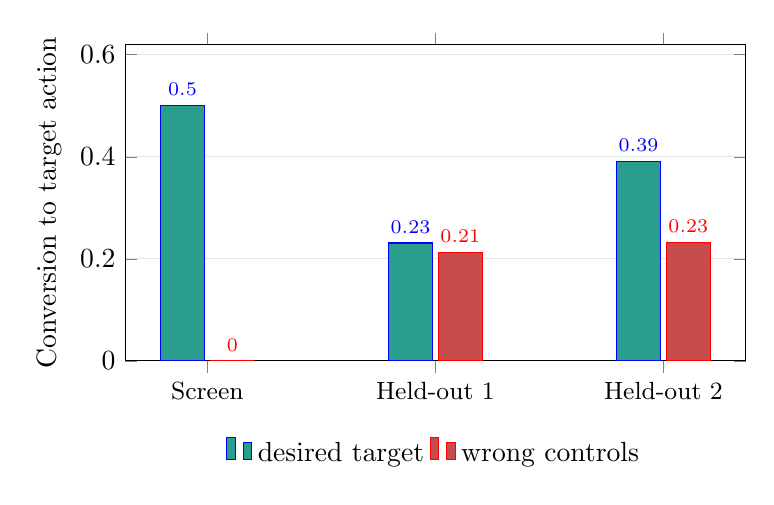
\begin{tikzpicture}
\begin{axis}[
  ybar,
  width=0.78\linewidth,
  height=5.6cm,
  ymin=0,
  ymax=0.62,
  ylabel={Conversion to target action},
  symbolic x coords={Screen,Held1,Held2},
  xtick=data,
  xticklabels={Screen,Held-out 1,Held-out 2},
  x tick label style={align=center,font=\small},
  bar width=16pt,
  enlarge x limits=0.18,
  legend style={draw=none,at={(0.5,-0.22)},anchor=north,legend columns=2},
  nodes near coords,
  nodes near coords style={font=\scriptsize},
  ymajorgrids=true,
  grid style={draw=gray!20}
]
\addplot+[fill=PlotTeal] coordinates {(Screen,0.500) (Held1,0.231) (Held2,0.391)};
\addplot+[fill=PlotRed] coordinates {(Screen,0.000) (Held1,0.212) (Held2,0.232)};
\legend{desired target, wrong controls}
\end{axis}
\end{tikzpicture}
\caption{Replication path for the successful Seed12 baseline-source steering condition. The first held-out run was marginal, so a larger confirmation was needed; the largest confirmation restores a clearer desired-vs-wrong separation.}
\label{fig:seed12_confirmation}
\end{figure}

The effect is not uniform across action labels.
In the largest confirmation, LEFT, RIGHT, and the small-sample UP target slices show positive desired-vs-control separation, while DOWN does not.
The correct interpretation is therefore a proof of principle for desired action steering, not a universal steering law for every action.

\begin{table}[t]
\centering
\caption{Largest Seed12 desired-vs-wrong confirmation for raw action-vs-baseline steering.}
\label{tab:seed12_confirm}
\begin{tabular}{lrrr}
\toprule
Group & Pairs & Conversions to desired & Conversion rate \\
\midrule
Desired target direction & 69 & 27 & 0.391 \\
Wrong target controls & 138 & 32 & 0.232 \\
\midrule
Advantage & & & +0.159 \\
\bottomrule
\end{tabular}
\end{table}

\begin{table}[t]
\centering
\small
\caption{Layer-23 retry and stress tests for the successful Seed12 raw action-vs-baseline protocol. Conversion means a baseline nonoptimal output becomes an A*-optimal desired action; wrong controls are nonoptimal candidate directions tested on the same prompt, seed, and source action.}
\label{tab:seed12_layer23_retry}
\begin{tabular}{p{0.32\linewidth}rrrrr}
\toprule
Layer/setting & Desired & Wrong & Desired conv. & Wrong conv. & Adv. \\
\midrule
Layer 15, $\alpha=0.5$ confirmation & 69 & 138 & 0.391 & 0.232 & +0.159 \\
Layer 23, $\alpha=0.5$ retry & 58 & 116 & 0.000 & 0.000 & 0.000 \\
Layer 23, each $\alpha\in\{1,2,4,8\}$ & 15 & 30 & 0.000 & 0.000 & 0.000 \\
Layer 23, each $\alpha\in\{32,64,128,256,512\}$ & 15 & 30 & 0.000 & 0.000 & 0.000 \\
Layer 23, $\alpha=-1024$ screen & 15 & 30 & 0.200 & 0.033 & +0.167 \\
Layer 23, $\alpha=-1024$ independent confirmation & 33 & 66 & 0.242 & 0.136 & +0.106 \\
\bottomrule
\end{tabular}
\end{table}

\begin{figure}[t]
\centering
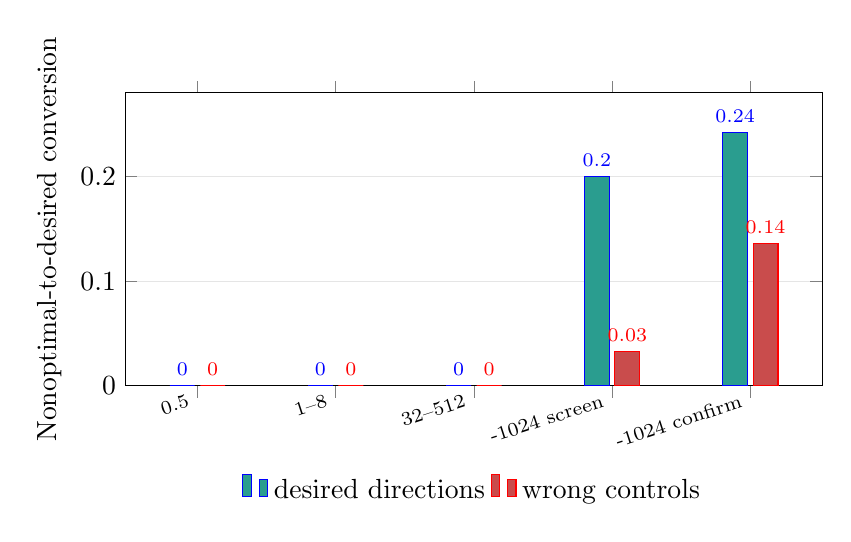
\begin{tikzpicture}
\begin{axis}[
  ybar,
  width=0.86\linewidth,
  height=5.3cm,
  ymin=0,
  ymax=0.28,
  ylabel={Nonoptimal-to-desired conversion},
  symbolic x coords={a0,a1,a2,a3,a4},
  xtick=data,
  xticklabels={0.5,1--8,32--512,-1024 screen,-1024 confirm},
  x tick label style={align=center,font=\scriptsize,rotate=18,anchor=east},
  bar width=9pt,
  enlarge x limits=0.13,
  legend style={draw=none,at={(0.5,-0.28)},anchor=north,legend columns=2},
  nodes near coords,
  nodes near coords style={font=\scriptsize},
  ymajorgrids=true,
  grid style={draw=gray!20}
]
\addplot+[fill=PlotTeal] coordinates {(a0,0.000) (a1,0.000) (a2,0.000) (a3,0.200) (a4,0.242)};
\addplot+[fill=PlotRed] coordinates {(a0,0.000) (a1,0.000) (a2,0.000) (a3,0.033) (a4,0.136)};
\legend{desired directions, wrong controls}
\end{axis}
\end{tikzpicture}
\caption{Layer-23 Seed12 action-margin regimes. Positive and matched alphas are inert, while the extreme opposite-sign stress setting shows a weaker desired-vs-wrong separation.}
\label{fig:seed12_layer23_stress}
\end{figure}

\FloatBarrier

\section{Discussion}

\subsection{What the Belief--Action Gap Is}

The results support a belief--action gap, but the gap is not simply ``the model lacks the right belief.''
The model often has the right information in a decodable form.
In fourroom, optimal actions are almost linearly recoverable from layer-15 prompt-suffix activations, while the observed actions are not.
In Seed12, optimal actions remain substantially decodable even under held-out-state averaging, although the model's recorded actions are rarely optimal.

The stronger interpretation is that there are multiple channels between representation and action.
Some activations encode task structure.
Some later computation may ignore, override, or rederive that structure.
Some prompt formats place a belief representation directly on the action channel; others route through verbose reasoning where the same representation may be only a correlate.
This explains why final-channel steering succeeds while the clean verbose flag-swap is null.
Even within final-channel steering, however, the success is not layer-general: layers 7 and 15 do not pass the same bidirectional steering test, while layer 23 does.
The Seed12 action-margin result shows the complementary point: the clean moderate-scale desired-action margin is layer-15-specific under the tested protocol, while layer 23 requires an extreme opposite-sign stress setting to show a weaker desired-vs-wrong effect.

\subsection{Why Decodability Is Not Causality}

A probe can decode a feature for at least three reasons.
The feature may be causally used by the model.
It may be a side effect of another variable that is causally used.
Or it may be recoverable because the hidden state contains enough world-state information for an external classifier to compute it, even if the model's own action head does not rely on that feature at that location.
The flag-swap results favor the second or third explanation for layer-15 \texttt{carrying\_key} at the final suffix positions in the corrected verbose prompt.

The Seed12 steering work also shows why directionality matters.
Changing an action is not enough: the strongest valid evidence compares a desired target direction against wrong target directions under the same prompt, same seed, and same baseline source action.
Only the source-aligned raw margin passes that test.
This is a sharper causal standard than measuring total action-change rate.

\subsection{Why Source Alignment Matters}

The failure of recorded-true-source steering is informative.
The recorded trajectory action is not always the model's current sampled action under the paired seed.
If the intervention is meant to move the output from what the model would actually do toward an optimal action, the source direction should be the model's actual baseline output, not a historical label.
The successful $W_t - W_s$ intervention uses exactly that source.
This suggests that action steering is local in logit-geometry terms: the useful direction depends on the current basin of the model's sampled action.
The layer-23 retry sharpens this claim.
Late-layer steering can be effective in final-channel \texttt{has\_key} prompts, but the same layer is not automatically best for Seed12 action-margin steering.
Layer 23 is inert over the matched and positive Seed12 alpha ranges, then becomes directional only at $\alpha=-1024$.
The useful layer and scale depend on both the represented variable and the prompt/action pathway being intervened on.

\subsection{Role of the IRL Experiments}

The fixed-grid MaxEnt IRL work is less central to the causal claim, but it supports the same picture at the behavioral modeling level.
In a fixed 13x13 key-door grid with 4,134 transitions, a structured reward model can describe long-horizon key-door-goal dependencies.
However, the neural-probe features for key and door beliefs were unavailable in that experiment, so the reported IRL features used binary fallbacks.
The IRL results should therefore be treated as task-structure context rather than direct evidence about hidden belief causality.

\section{Limitations}

Several limitations remain.
First, the clean flag-swap run has only 30 samples per condition and high parse-fail rates, so it rules out a large effect but not a small one.
Second, the flag-swap causal conclusion is localized to layer 15 and final suffix positions in one corrected verbose door-key prompt.
Third, final-channel steering uses synthetic matched prompt families and large layer-23 scales, so it may overstate how easily belief directions steer natural verbose reasoning.
Fourth, the strongest clean Seed12 desired steering result is on a balanced 12-step subset, not the full eligible Seed12 sweep, and the DOWN target slice fails to show positive desired-vs-control advantage.
Fifth, the layer-23 Seed12 effect appears only at the extreme opposite-sign stress scale $\alpha=-1024$, where wrong controls also sometimes convert to optimal actions; it should be treated as weaker evidence than the layer-15 alpha-0.5 confirmation.
Sixth, all steering results use sampled decoding, so seed control and paired baselines are essential.

\section{Future Work}

The next experiments should target the remaining uncertainty rather than repeat already-settled variants.
A layer-position sweep for the corrected flag-swap prompt should test the \texttt{True}/\texttt{False} token position, all 19 suffix positions, and later layers such as 23.
A multi-cell corrected flag-swap sweep would test whether the null generalizes beyond the door-adjacent cell.
For Seed12, the raw baseline-source margin should be scaled to more steps and analyzed per target action, especially DOWN.
The layer-23 $\alpha=-1024$ stress result should be repeated on a larger held-out set and bracketed with nearby negative alphas to determine whether it is a narrow threshold or a broader late-layer regime.
Finally, a non-adaptive version could estimate the baseline source action from a probe or from a preliminary low-cost pass, preserving the causal source-alignment insight while reducing the need for a no-hook generation for every sample.

\section{Conclusion}

The experiments support a precise version of the belief--action gap.
GPT-OSS-20B gridworld activations often encode the state or optimal action more clearly than the model's sampled actions reveal.
But encoded information is not necessarily load-bearing for action under a given intervention.
Clean causal evidence requires directional controls, not just action changes.
Under those controls, belief/action steering is possible in matched final-channel settings and in Seed12 when the intervention is aligned to the model's actual baseline action.
The Seed12 results are not layer-monotonic: layer 15 gives the cleaner moderate-scale action-margin effect, while layer 23 only gives a weaker effect at an extreme opposite-sign scale.
The best current model is therefore not ``beliefs do not matter,'' but rather: decodable beliefs become actions only when the representation lies on the active action pathway for the prompt, layer, position, and source state being intervened on.

\begin{thebibliography}{9}

\bibitem{alain2016}
Guillaume Alain and Yoshua Bengio.
\newblock Understanding intermediate layers using linear classifier probes.
\newblock \emph{arXiv:1610.01644}, 2016.

\bibitem{belinkov2022}
Yonatan Belinkov.
\newblock Probing classifiers: Promises, shortcomings, and advances.
\newblock \emph{Computational Linguistics}, 48(1):207--219, 2022.

\bibitem{hewitt2019}
John Hewitt and Percy Liang.
\newblock Designing and interpreting probes with control tasks.
\newblock In \emph{Proceedings of EMNLP-IJCNLP}, 2019.

\bibitem{meng2022}
Kevin Meng, David Bau, Alex Andonian, and Yonatan Belinkov.
\newblock Locating and editing factual associations in GPT.
\newblock In \emph{Advances in Neural Information Processing Systems}, 2022.

\bibitem{pearl2009}
Judea Pearl.
\newblock \emph{Causality: Models, Reasoning, and Inference}.
\newblock Cambridge University Press, 2nd edition, 2009.

\bibitem{turner2023}
Alexander Matt Turner, Lisa Thiergart, Gavin Leech, David Udell, Juan J. Vazquez, Ulisse Mini, and Monte MacDiarmid.
\newblock Activation addition: Steering language models without optimization.
\newblock \emph{arXiv:2308.10248}, 2023.

\bibitem{ziebart2008}
Brian D. Ziebart, Andrew L. Maas, J. Andrew Bagnell, and Anind K. Dey.
\newblock Maximum entropy inverse reinforcement learning.
\newblock In \emph{Proceedings of AAAI}, 2008.

\end{thebibliography}

\appendix
\section{Artifact Pointers}

The main source reports and artifacts are:
\begin{sloppypar}
\begin{itemize}[leftmargin=*]
  \item \path{results/fourroom_episode_sweep_T0_agent_vs_optimal_results.md}
  \item \path{reports/seed12_action_probes/seed12_action_probe_report.md}
  \item \path{results/flag_swap_results.md}
  \item \path{flag_swap/simple_corridor/final_channel_policy_last3/probe_family_matched/report.md}
  \item \path{flag_swap/door_key_grid/final_channel_last3_v2/probe_family_matched/report.md}
  \item \path{reports/seed12_optimal_action_steering/detailed_report/seed12_desired_direction_steering_detailed_report.md}
  \item \path{reports/fixed_grid_maxent_irl_report.md}
\end{itemize}
\end{sloppypar}

\end{document}
